%DS0



\section{ĐỀ SỐ \thesection }
\setcounter{bt}{0}
%%Câu 1.
\begin{bt}Thực hiện phép tính:
	\begin{listEX}[3]
		\item $(-33) + 45 + (-67)$;
		\item $28\cdot 69 + 28\cdot 31 + (-100)$;
		\item $75:\left[ (153 - 6\cdot 5^2)\cdot 8 + 2011^0\right] $.
	\end{listEX}
	\loigiai{
		\begin{listEX}[3]
			\item $(-33) + 45 + (-67)$\\
				$= 45 - 33 - 67$\\
				$= 12 - 67$\\
				$= -55$ 
			\item $28\cdot 69 + 28\cdot 31 + (-100)$\\
				$= 28(69 + 31) - 100$\\
				$= 28\cdot 100 - 100$\\
				$= 2800 - 100$
				$= 2700$ 
			\item $75:\left[ (153 - 6\cdot 5^2)\cdot 8 + 2011^0\right]$\\
				$= 75:\left[(153 - 150)\cdot 8 + 1\right]$\\
				$= 75:(3\cdot 8 + 1)$\\
				$= 75:25$
				$= 3$ 
		\end{listEX}
	}
\end{bt}


%%Câu 2.
\begin{bt} Tìm số nguyên $x$, biết
	\begin{listEX}[3]
		\item $6x + 15 = 75$;
		\item $x - 12 = -27$;
		\item $23 + (x - 5):4 = 3^8 :3^5$.
	\end{listEX}
	\loigiai{
		\begin{listEX}[3]
			\item $6x + 15  = 75$\\
				\hspace{2 cm}$\begin{aligned} 
				6x &= 75 - 15\\
				6x &= 60\\
				x &= 10
				\end{aligned}$ 
			\item 	$x - 12  = -27$\\
				\hspace{2 cm}$\begin{aligned} 
				x &= -27 + 12\\
				x &= -15
				\end{aligned}$ 
			\item $23 + (x - 5):4  = 3^8 : 3^5$\\
				\hspace{1 cm}$\begin{aligned} 
				23 + (x - 5):4 &= 3^3\\
				23 + (x - 5):4 &= 27\\
				(x - 5):4 &= 4\\
				x - 5 &= 16\\
				x &= 21
			\end{aligned}$
		\end{listEX}
		
	}
\end{bt}

%%Câu 3.
\begin{bt}
	Học sinh khối $6$ có $180$ bạn nữ và $102$ bạn nam tham gia văn nghệ. Cô phụ trách muốn chia ra thành các nhóm sao cho số nam và nữ mỗi nhóm đều bằng nhau. Hỏi có thể chia nhiều nhất bao nhiêu nhóm? Mỗi nhóm có bao nhiêu nam, bao nhiêu nữ?
	\loigiai{
		Gọi $x$ là số nhóm nhiều nhất có thể chia $(x\in \mathbb N)$\\
		$x =$ ƯCLN$(180;102)$
		
		$180=2^2\cdot 3^2\cdot 5\qquad  102=2\cdot 3\cdot 17$
		
		ƯCLN$(180;102)=2\cdot 3=6$\\
		Vậy có thể chia nhiều nhất 6 nhóm.
		Mỗi nhóm có $30$ bạn nữ và $17$ bạn nam.
	}
\end{bt}


%%Câu 4.
\begin{bt}
	\immini[thm]{Bác Hai có một mảnh vườn hình chữ nhật với chiều dài $30$ m và chiều rộng là $12$ m. Giữa mảnh vườn, bác đào một cái ao hình vuông để nuôi cá có độ dài cạnh $9$ m, phần còn lại của mảnh vườn bác dùng để trồng rau.
		\begin{enumerate}
			\item Tính diện tích trồng rau.
			\item Bác Hai đi mua hạt giống để trồng rau, biết cần gieo $20$ gram hạt giống trên 1 m$^2$ đất. Hỏi cần bao nhiêu gram hạt giống đề gieo hết phần đất trồng rau?
		\end{enumerate}
	}
	{
		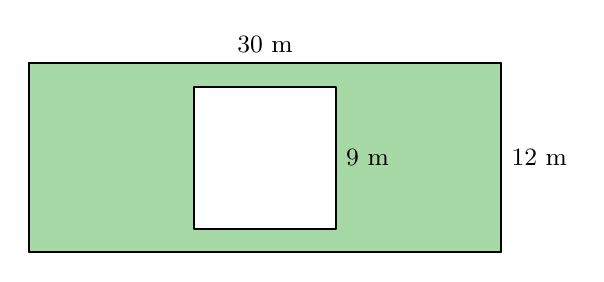
\begin{tikzpicture}[scale=1,line width=0.8pt,line join=round,>=stealth,font=\small]
			\def\s{5}
			;
			\draw[fill=white] (0,0) rectangle (30/\s,12/\s);
			\draw[fill=green!40!gray!50] (0,0) rectangle (30/\s,12/\s);
			\draw[fill=white] (10.5/\s,1.5/\s) rectangle (19.5/\s,10.5/\s); 
			\draw
			(19.5/\s,6/\s) node[right]{9 m}
			(30/\s,6/\s) node[right]{12 m}
			(15/\s,12/\s) node[above]{30 m}
			;
		\end{tikzpicture}
	}
	\loigiai{
		\begin{enumerate}
			\item Diện tích trồng rau là: $30\cdot12 - 9\cdot9 = 279$ (m$^2$).
			\item Số gram hạt giống cần để gieo hết phần đất trồng rau là: $20\cdot279 = 5\,580$ (g).
		\end{enumerate}
	}
\end{bt}


%%Câu 5.
\begin{bt}Một nhà sách nhập về một lô hàng gồm $40$ cái máy tính Casio-FX$570$ với giá $14\,000\,000$ đồng và bán ra với giá $400\,000$ đồng một máy. Sau khi bán được $20$ cái máy tính thì nhà sách giảm giá còn $380\,000$ đồng/máy và bán hết số máy tính còn lại. Hỏi nhà sách lời hay lỗ bao nhiêu tiền khi bán hết lô hàng trên?
	
	\loigiai{
		Số tiền thu được khi bán 20 cái máy tính đầu tiên là: 
			$20 \cdot 400\,000 = 8\,000\,000$ (đồng)
			
		Số tiền thu được khi bán hết số máy tính còn lại là: 
			$20 \cdot 380\,000 = 7\,600\,000$ (đồng)
			
		Số tiền nhà sách thu được khi bán hết 40 cái máy tính là: 
			$8\,000\,000 + 7\,600\,000 = 15\,600\,000$ (đồng)
			
		Vì $15\,600\,000$ đồng $> 14\,000\,000$ đồng nên nhà sách lời.
		 
		Số tiền nhà sách lời là: $15\,600\,000 - 14\,000\,000 = 1\,600\,000$ (đồng)
	}
\end{bt}


%%Câu 6.
\begin{bt} Tìm số nguyên tố $n$ sao cho $(3n+7)$ là bội của $(n+1)$.  
	
	\loigiai{Để $(3n+7)$ là bội của $(n+1)$ thì $(3n+7)$ phải chia hết cho $(n+1)$.\\
		Ta có: $3n+7 = 3(n+1) + 4$
		
		Để $3n+7$ chia hết cho $n+1$ thì $4$ phải chia hết cho $n+1$.
		
		Điều này có nghĩa là $(n+1)$ là ước của $4$.
		
		$(n+1)\in$Ư$(4)=\{\pm1, \pm2, \pm4\}$.
	$	\Rightarrow  n\in \{-5;-3;-2;0;1;3\}$\\
		Nên số nguyên tố $n$ thỏa mãn đề bài là $n = 3$.}
	
\end{bt}




